\section{The Kernel}

These are the main functions of any operating system. Commonly they are refereed to from a designer's view, but the user's view can be much more helpful to actually understand how it works.

\begin{center}
	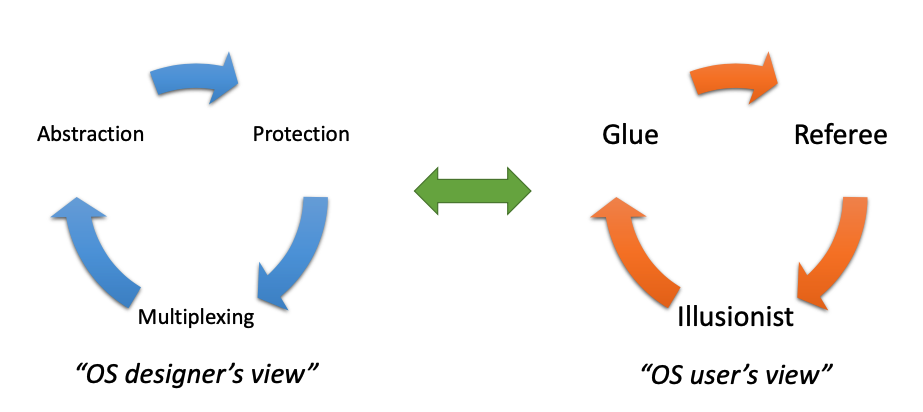
\includegraphics[width=\linewidth]{os-functions.png}
\end{center}


\subsection{Bootstraping}

The term bootstraping referees to pulling himself up from his own boots. In computer systems it is why we call the process of starting up a computer booting. This boot process looks like this:

\begin{enumerate}
	\item CPU starts executing code at a fixed address (Boot ROM)
	\item Boot ROM code loads 2nd stage boot loader into RAM
	\item Boot loader loads kernel and optionally initials file system into RAM
	\item Jumps to kernel entry point
\end{enumerate}

The first few lines are always written in assembly, but generally we want to switch to C as soon as possible.


\subsection{Mode Switch}

One of our main goals is to protect the OS from applications that could harm it (intentionally or not). For this purpose we introduce two different modes:

\begin{itemize}
	\item Kernel mode - execution with full privileges, read/write to any memory, access and I/O, etc. code here must be carefully written
	\item User mode - limited privileges, only those granted by the OS kernel
\end{itemize}

These two (or more) modes are already implemented in hardware. The main reason for a mode switch is when we encounter a processor exception (mode switch from user to kernel mode). If this is the case, we want the following to happen:

\begin{enumerate}
	\item Finish executing current instruction
	\item Switch mode from user to kernel
	\item Look up exception cause in exception vector table
	\item Jump to this address
\end{enumerate}

Further we may also want to save the registers and switch page tables. When switching between the modes we also have to change our address space, but we might want to access some informations from the user mode address space. One way of doing this is to use a so called \textbf{trampoline}, this is a part of the address space that gets mapped to the same location in user and kernel mode.

\begin{center}
	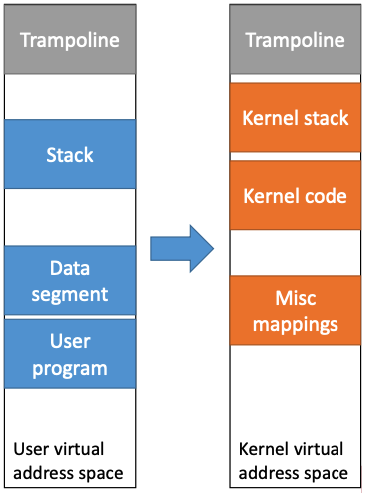
\includegraphics[width=0.4\linewidth]{trampoline.png}
\end{center}

Mode switches can also occur the other way around (from kernel mode to user mode). The mains reasons for this are:

\begin{itemize}
	\item New process / thread start
	\item Return from exception
	\item Process / thread context switch
	\item User-level upcall (UNIX signal)
\end{itemize}

This leads us to the following perspective:

\begin{center}
	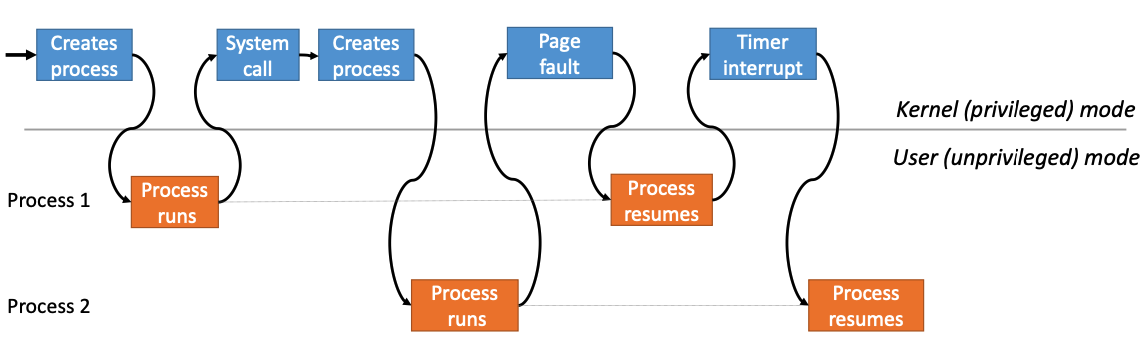
\includegraphics[width=\linewidth]{mode-switch.png}
\end{center}

The mode switch is fundamental to modern computers:

\begin{itemize}
	\item It enables virtualization of the processor
	\item It creates the illusion of multiple computers
	\item It referees access to the CPU
\end{itemize}


\subsection{General Model of OS Structure}

\begin{center}
	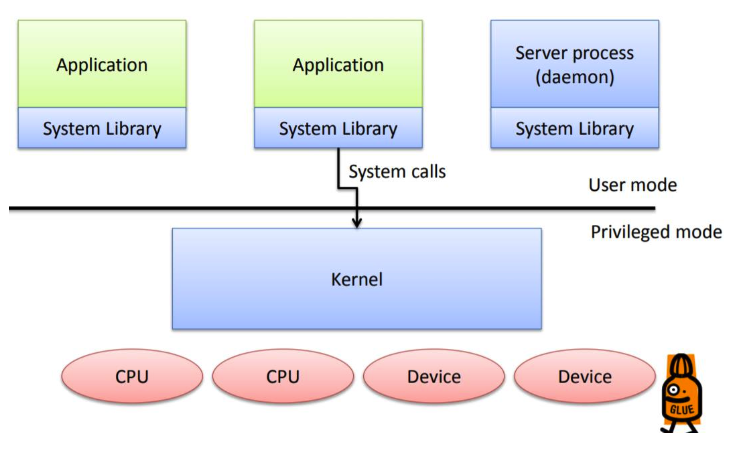
\includegraphics[width=0.9\linewidth]{os-structure.png}
\end{center}

\begin{itemize}
	\item Kernel - code that runs in kernel mode
	\item System Library - interface to kernel, enough for most programs
	\item Daemon - user space process which provides OS services, varying levels of privileges
\end{itemize}

We can differentiate between monolithic kernels and microkernels, depending on the amount of code in kernel mode.


\subsection{System Calls}

System calls are the only way for user mode programs to enter kernel mode. System calls are a type of exception, but they try to look a lot more like a procedure call. Therefore the kernel system call handler has to first locate arguments, copy these arguments into kernel memory, validate these arguments and the copy the results back into user memory after execution. An example of such a system call would be \textit{write()}. 


\subsection{Hardware Timers}

What happens if a user mode program does not cause any exception and does not give control back to the kernel? Hardware timers are a solution for this problem, the hardware device periodically interrupts the processor and returns control to the kernel handler, which sets the time of the next interrupt.
